\section{GamingReplay}

A empresa especializa-se na venda/compra de artigos relacionados com videojogos desde consolas,videojogos de varias consolas como támbem Merchandising.Está no mercado desde 2009 mas com experiência desde 2007 nesta área.

A marca é comercializada por \emph{SharingJourney,Lda} como pode ser retirado na figura seguinte retirada do Website.Apesar de a Gamingreplay estar no mercado desde 2009 a empresa que a comercializa foi oficialmente constituida em 21 de Junho de 2013.

\begin{figure}[h!]
\caption{Informação da Empresa}
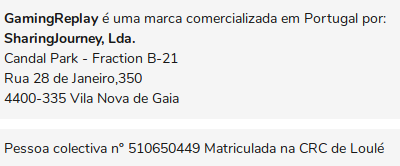
\includegraphics{Images/LocEmpresa.png}
\end{figure}

\subsection{Localização \& Contactos}

Esta pequena empresa tem duas lojas fisicas localizadas em \emph{Arrábida Shopping Piso 1 - Loja 166 - Vila Nova de Gaia} e em \emph{Almada Forúm Piso 0 - Loja 1.112 - Almada} para além disso também gerem um Website que funciona como loja Online em \emph{https://www.gamingreplay.pt}(Falta Referencia a Imagem).
\begin{figure}[h!]
\caption{Localização da Empresa}
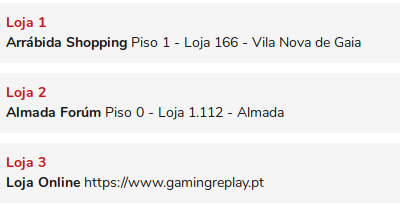
\includegraphics{Images/LocLojas.png}
\end{figure}
Ainda sobre a loja online ainda pode descubrir-se um Código Postal associado (4400-275).

A primeira loja tem associada um email \emph{lojaarrabida@gamingreplay.com}
como um telefone \emph{224 103 675}.E o mesmo encontra-se sobre a segunda loja \emph{lojaalmada@gamingreplay.com -265 414 909}.Enquanto a loja online esta tambem tem um email \emph{clientes@gamingreplay.com} eum telemovel associado \emph{919 176 465}.

\subsection{Política de privacidade}

A política de privacidade que consta a empresa estar conforme é a que está prevista no \emph{Regulamento (UE) 2016/679} do Parlamento Europeu e do Conselho de 27 de Abril de 2016.

Os dados pessoais(nome,e-mail,telefone,morada) dos clientes são guardados pelo período de 2 anos desde o consentimento pelo mesmo.Caso o cliente usufrua de algum serviço da empresa o prazo sera extendido para 5 anos.O utilizador tem o direito de realizar as seguintes operações indicadas na figura seguinte.

\begin{figure}[h!]
\caption{Operações do Cliente sobre os seus dados}
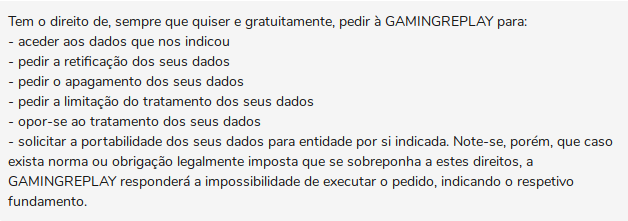
\includegraphics{Images/OperCliente.png}
\end{figure}

\subsection{Dominios Associados}

O website \emph{www.gamingreplay.com} é utilizado como a página principal do negócio, porém ao pesquisar os A records associados(Referencia a imagem) a esse mesmo dominio encontramos o seguinte:

\begin{enumerate}

\item Os dominios que contem "media" redirecionam para a página principal.Possivelmente sejam vários servidores para previnir ataques de Denial of Service.

\item O dominio começado por "phpma" corresponde a uma pagina administração de base de dados.Mais especificamente, corresponde a um software phpMyAdmin que permite gerir base de dados MySQL atráves da Web.Para aceder a base de dados é necessário um par username/password.

\item O dominio webdisk.gamingreplay.com corresponde á um serviço de gestao de ficheiros usados pelo website.Requere autentificação para aceder ao serviço

\item O dominio cpanel.gamingreplay.com diz respeito a um serviço de gestao do Website onde pode estar integrado o serviço anterior.Como os anteriores requere autentificação.

\item O dominio webmail.gamingreplay.com tanto como o autodiscover.gamingreplay.com fornecem serviços de gestão e-mail.O primeiro está integrado no Cpanel e o segundo é um serviço necessário para usar o Outlook Exchange.

\item O dominio gamingreplayserver.gamingreplay.com provavelmente diz respeito ao back-end da página.Encontra-se em Lisboa e o serviço responsável por esse IP é a empresa \emph{Claranet Portugal}.

\end{enumerate}

Note-se que todos estes dominios excepto o ultimo estão localizados no mesmo IPv4.

\begin{figure}[h!]
\caption{A records associados a Gamingreplay.com}
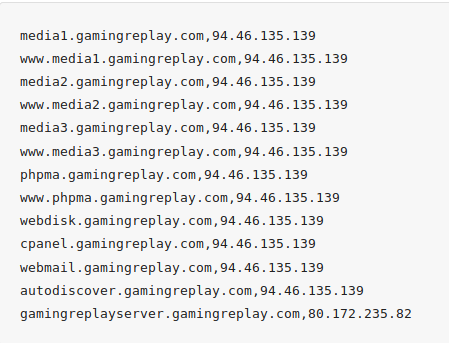
\includegraphics{Images/DNSArecords.png}
\end{figure}

Observando outros tipos de DNS records(Referencia a imagem) pode concluir-se tambem que:

\begin{enumerate}

\item Os servidores DNS que estão responsaveis pelo domínio pertence a empresa linxisp sendo o ns1.linxisp.net o servidor primário.

\item No record TXT encontra-se dois IPs um corresponde ao IP associado ao Website.O outro corresponde a um serviço de Cloud da empresa \emph{Almouroltec - Serviços Informática Internet, Lda.}.Este formato de record Txt corresponde a um Sender Policy Framework ,isto é, os IPs que podem enviar emails atraves do dominio de forma a autentificar a origem do email e este não ser considerado como spam.

\end{enumerate}

\begin{figure}[h!]
\caption{DNS records associados a Gamingreplay.com}
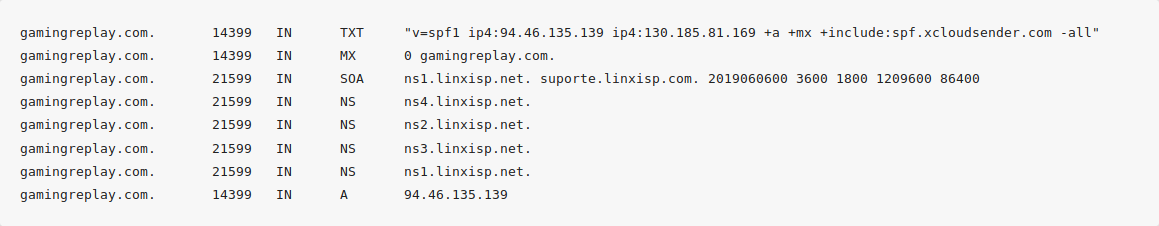
\includegraphics{Images/DNSRecords.png}
\end{figure}




